\documentclass[border=3pt]{standalone}
% Preâmbulo compartilhado pelos diagramas TikZ da aula 6 de IHC (Necessidades e Requisitos)
\usepackage[T1]{fontenc}
\usepackage[utf8]{inputenc}
\usepackage{lmodern}
\usepackage{amsmath}
\usepackage{xcolor}
\usepackage{tikz}
\usetikzlibrary{arrows.meta,angles,quotes,decorations.pathmorphing,calc,
                positioning,shapes.geometric,shapes.misc,backgrounds,fit,
                math}

% Paleta (mesma dos SVGs originais)
% Paleta da disciplina de IHC: acento roxo (#755099), da capa do livro.
% (o nome "dblue" é mantido para não alterar todos os diagramas)
\definecolor{dblue}{HTML}{755099}
\definecolor{dorange}{HTML}{B3541E}
\definecolor{dgreen}{HTML}{4A7C59}
\definecolor{dred}{HTML}{9C4B4B}
\definecolor{dcream}{HTML}{F4F1EA}
\definecolor{dshade}{HTML}{DDD7C9}

% Função gaussiana (não normalizada por padrão de escala visual)
\pgfmathdeclarefunction{gauss}{3}{%
  \pgfmathparse{1/(#3*sqrt(2*pi))*exp(-((#1-#2)^2)/(2*#3^2))}%
}

% Estilos comuns (prefixo d... para não colidir com chaves internas do pgf)
\tikzset{
  >={Stealth[length=2mm]},
  dguide/.style={gray!55, dashed, line width=0.4pt},
  daxis/.style={gray!60, line width=0.7pt, ->},
  dbody/.style={fill=black!3, draw=black!80, line width=1pt},
  dacc/.style={draw=dblue, line width=1pt},
  dlbl/.style={black!55, font=\small},
  dsub/.style={black!45, font=\footnotesize},
  dstate/.style={circle, draw=black!80, fill=dcream, line width=1pt,
                 minimum size=17mm, font=\large, inner sep=1pt},
  dobs/.style={circle, draw=black!80, fill=dshade, line width=1pt,
               minimum size=14mm, font=\large, inner sep=1pt},
  dbox/.style={rounded corners=2pt, draw=black!80, fill=dcream, line width=1pt,
               align=center, inner sep=6pt},
  dop/.style={circle, draw=black!80, fill=white, line width=1pt,
              minimum size=6mm, inner sep=0pt, font=\small},
  dtrans/.style={->, dblue, line width=1pt},
  dmeas/.style={->, dorange, line width=1pt},
  dcurve/.style={line width=1pt, dblue},
  dcurveb/.style={line width=1.4pt, dorange},
}

\begin{document}
\hyphenpenalty=10000 \exhyphenpenalty=10000 \tolerance=9999 \emergencystretch=3em
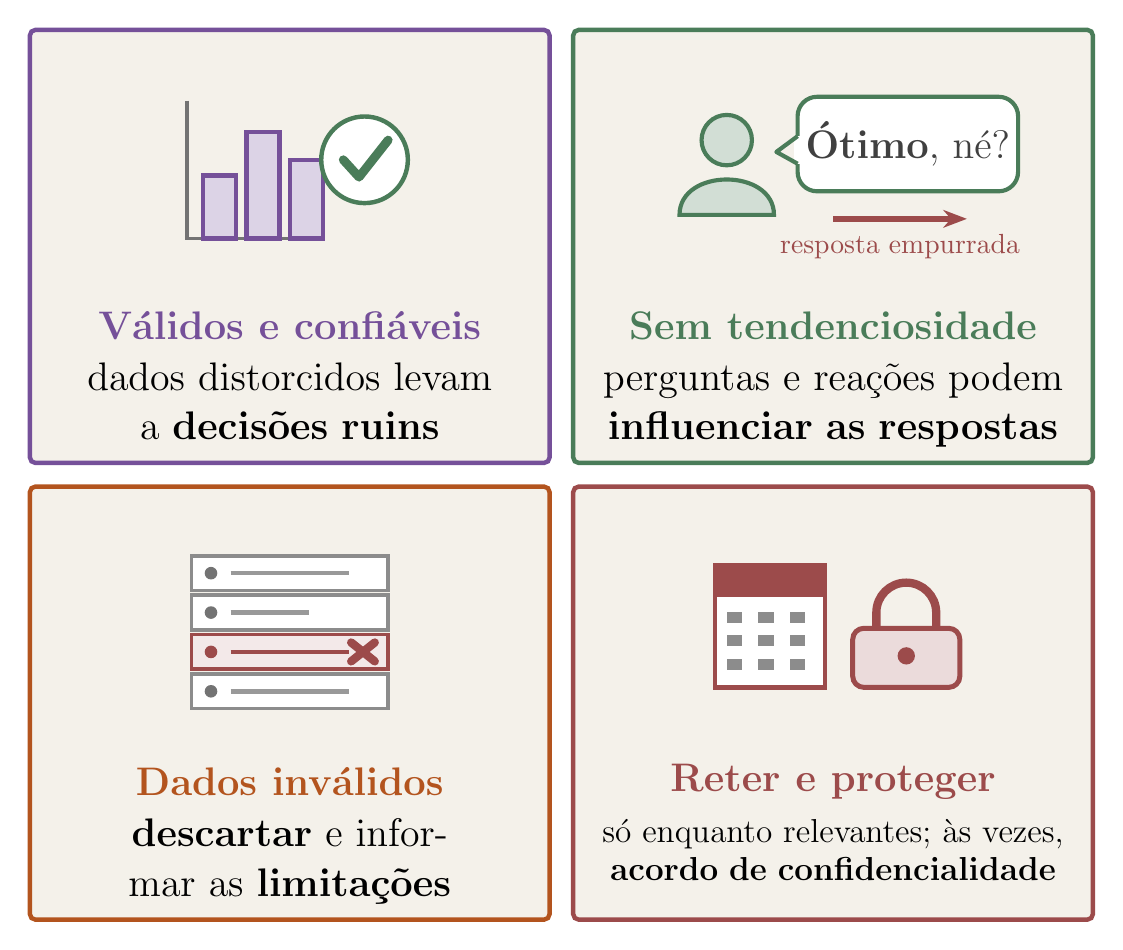
\begin{tikzpicture}[x=1cm,y=1cm]
\node[dbox, draw=dblue, line width=1.6pt, minimum width=6.6cm, minimum height=5.5cm] at (3.30,8.55) {};
\node[font=\Large\bfseries, dblue] at (3.30,7.55) {Válidos e confiáveis};
\node[font=\Large, text width=6.0cm, align=center, anchor=north] at (3.30,7.20) {dados distorcidos levam a \textbf{decisões ruins}};
\draw[black!55, line width=1.4pt] (2.00,10.40) -- (2.00,8.65) -- (3.70,8.65);
\draw[dblue, fill=dblue!25!white, line width=1.5pt] (2.20,8.65) rectangle ++(0.42,0.80);
\draw[dblue, fill=dblue!25!white, line width=1.5pt] (2.75,8.65) rectangle ++(0.42,1.35);
\draw[dblue, fill=dblue!25!white, line width=1.5pt] (3.30,8.65) rectangle ++(0.42,1.00);
\draw[dgreen, fill=white, line width=1.6pt] (4.25,9.65) circle (0.55);
\draw[dgreen, line width=3.2pt, line cap=round, line join=round] (3.98,9.65) -- (4.18,9.43) -- (4.55,9.90);
\node[dbox, draw=dgreen, line width=1.6pt, minimum width=6.6cm, minimum height=5.5cm] at (10.20,8.55) {};
\node[font=\Large\bfseries, dgreen] at (10.20,7.55) {Sem tendenciosidade};
\node[font=\Large, text width=6.0cm, align=center, anchor=north] at (10.20,7.20) {perguntas e reações podem \textbf{influenciar as respostas}};
\fill[dgreen!25!white, draw=dgreen, line width=1.5pt] (8.85,9.90) circle (0.32);
\fill[dgreen!25!white, draw=dgreen, line width=1.5pt] (8.25,8.95) .. controls (8.25,9.55) and (9.45,9.55) .. (9.45,8.95) -- cycle;
\draw[dgreen, fill=white, line width=1.5pt, rounded corners=7pt] (9.75,9.25) rectangle (12.55,10.45);
\draw[white, line width=2.6pt] (9.75,9.60) -- (9.75,9.95);
\draw[dgreen, line width=1.5pt, line join=round] (9.75,9.60) -- (9.48,9.75) -- (9.75,9.95);
\node[font=\Large, black!75] at (11.15,9.85) {\textbf{Ótimo}, né?};
\draw[dred, line width=2pt, -{Stealth[length=3mm]}] (10.20,8.90) -- (11.90,8.90);
\node[font=\normalsize, dred, anchor=north] at (11.05,8.83) {resposta empurrada};
\node[dbox, draw=dorange, line width=1.6pt, minimum width=6.6cm, minimum height=5.5cm] at (3.30,2.75) {};
\node[font=\Large\bfseries, dorange] at (3.30,1.75) {Dados inválidos};
\node[font=\Large, text width=6.0cm, align=center, anchor=north] at (3.30,1.40) {\textbf{descartar} e informar as \textbf{limitações}};
\draw[black!45, fill=white, line width=1.3pt] (2.05,4.18) rectangle (4.55,4.62);
\fill[black!55] (2.30,4.40) circle (0.08);
\draw[black!40, line width=1.6pt] (2.55,4.40) -- ++(1.50,0);
\draw[black!45, fill=white, line width=1.3pt] (2.05,3.68) rectangle (4.55,4.12);
\fill[black!55] (2.30,3.90) circle (0.08);
\draw[black!40, line width=1.6pt] (2.55,3.90) -- ++(1.00,0);
\draw[dred, fill=dred!12!white, line width=1.3pt] (2.05,3.18) rectangle (4.55,3.62);
\fill[dred] (2.30,3.40) circle (0.08);
\draw[dred, line width=1.6pt] (2.55,3.40) -- ++(1.50,0);
\draw[black!45, fill=white, line width=1.3pt] (2.05,2.68) rectangle (4.55,3.12);
\fill[black!55] (2.30,2.90) circle (0.08);
\draw[black!40, line width=1.6pt] (2.55,2.90) -- ++(1.50,0);
\draw[dred, line width=3pt, line cap=round] (4.08,3.52) -- (4.38,3.28) (4.08,3.28) -- (4.38,3.52);
\node[dbox, draw=dred, line width=1.6pt, minimum width=6.6cm, minimum height=5.5cm] at (10.20,2.75) {};
\node[font=\Large\bfseries, dred] at (10.20,1.75) {Reter e proteger};
\node[font=\large, text width=6.0cm, align=center, anchor=north] at (10.20,1.40) {só enquanto relevantes; às vezes, \textbf{acordo de confidencialidade}};
\draw[dred, fill=white, line width=1.6pt] (8.70,2.95) rectangle (10.10,4.50);
\fill[dred] (8.70,4.10) rectangle (10.10,4.50);
\fill[black!45] (8.85,3.77) rectangle ++(0.2,0.14);
\fill[black!45] (9.25,3.77) rectangle ++(0.2,0.14);
\fill[black!45] (9.65,3.77) rectangle ++(0.2,0.14);
\fill[black!45] (8.85,3.47) rectangle ++(0.2,0.14);
\fill[black!45] (9.25,3.47) rectangle ++(0.2,0.14);
\fill[black!45] (9.65,3.47) rectangle ++(0.2,0.14);
\fill[black!45] (8.85,3.17) rectangle ++(0.2,0.14);
\fill[black!45] (9.25,3.17) rectangle ++(0.2,0.14);
\fill[black!45] (9.65,3.17) rectangle ++(0.2,0.14);
\draw[dred, line width=3pt] (10.75,3.65) -- (10.75,3.90) arc (180:0:0.38) -- (11.51,3.65);
\draw[dred, fill=dred!20!white, line width=1.8pt, rounded corners=4pt] (10.45,2.95) rectangle (11.81,3.70);
\fill[dred] (11.13,3.35) circle (0.11);
\end{tikzpicture}
\end{document}
